%!TEX root = main.tex
\section{System\label{sec:system}}
\subsection{System Architecture}
We have implemented \system\ as a Flask web application on top of a PostgreSQL database. In Figure~\ref{system_architecture}, we present the system architecture of \system, which consists of three core modules: the traversal module, the query module, and the statistics module. The interaction manager deals with the supported user interaction described in Section~\ref{sec:interaction} and sends a request to the lattice module which  contains several algorithms for generating and traversing the visualization lattice described in Section~\ref{sec:algorithms}. For generating the visualization lattice, the lattice module passes a list of data subsets corresponding to visualizations to be generated to the query module. The query module translates these visualizations into queries, and then optimizes (by grouping) and executes the queries. The statistics module is an optional module that allows the lattice module to prune low-utility visualizations without actually generating them. Specifically, it generates coarse statistics for the unexplored visualizations based on the current list of explored visualizations. Finally, the dashboard renderer takes the resulting visualizations to be included in the dashboard and perform any rendering preprocessing procedures for display and navigation of the dashboard as described in Section \ref{sec:navigation}.
\begin{figure}[ht!]
\centering
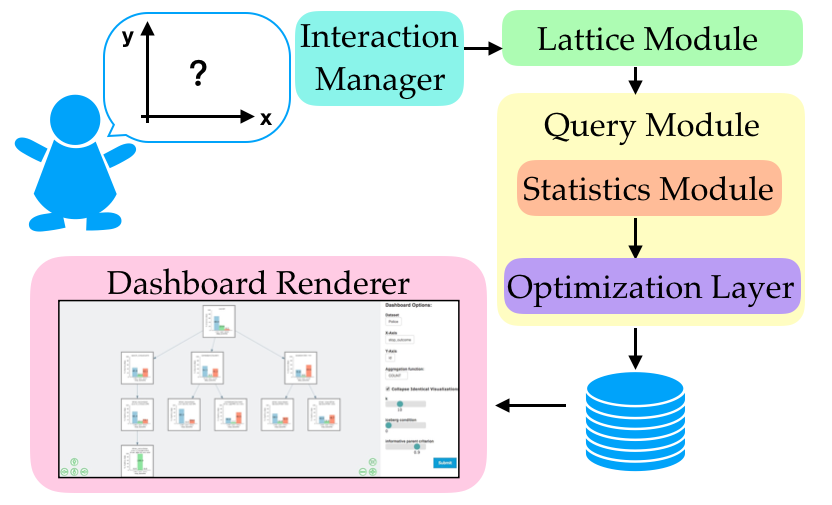
\includegraphics[width=\linewidth]{figures/system_architecture.png}
\caption{System Architecture of \system. User starts with x and y axes of interest and requests for $k$ visualizations in the dashboard. The request is processed by generating the lattice with the help of the querying module, visualization selection through the lattice traversal algorithms, and finally the dashboard is displayed at the frontend through the dashboard renderer. }%  The interaction manager translates the request to the traversal module that ???? [should we look at the offline case??]}
\label{system_architecture}
\end{figure}

\subsection{Algorithms\label{sec:algorithms}}
We give an overview of our algorithms by first discussing the approaches to generate the visualization lattice, and then presenting a high-level overview of our traversal algorithms.

\stitle{Lattice Generation.} Our system supports two variants of traversal algorithms based on the lattice generation procedure---offline variants that first generate the complete lattice and then work towards identifying the maximum utility solution, and online variants that incrementally generate the lattice and simultaneously identify the solution. The offline variants are appropriate for datasets with a small number of low-cardinality attributes, where we can generate the entire lattice in a reasonable time; whereas the online variants are appropriate for datasets with large number of high-cardinality attributes, where we incrementally generate a partial lattice.

%In most cases, the lattice contains a large number of visualizations due to the presence of many attributes or high-cardinality attributes in the dataset. In such cases finding an optimal solution is computationally challenging.

\stitle{Lattice Traversal.} Given the materialized lattice, the objective of the traversal algorithm is to find the connected subgraph in the lattice that has the maximum combined edge utility. Here, we discuss the \textit{frontier greedy} algorithm which is used for generating the dashboards for our user study and defer our discussion on the details of other algorithms that we have developed to the technical report.
% \begin{figure}[ht!]
% \centering
% 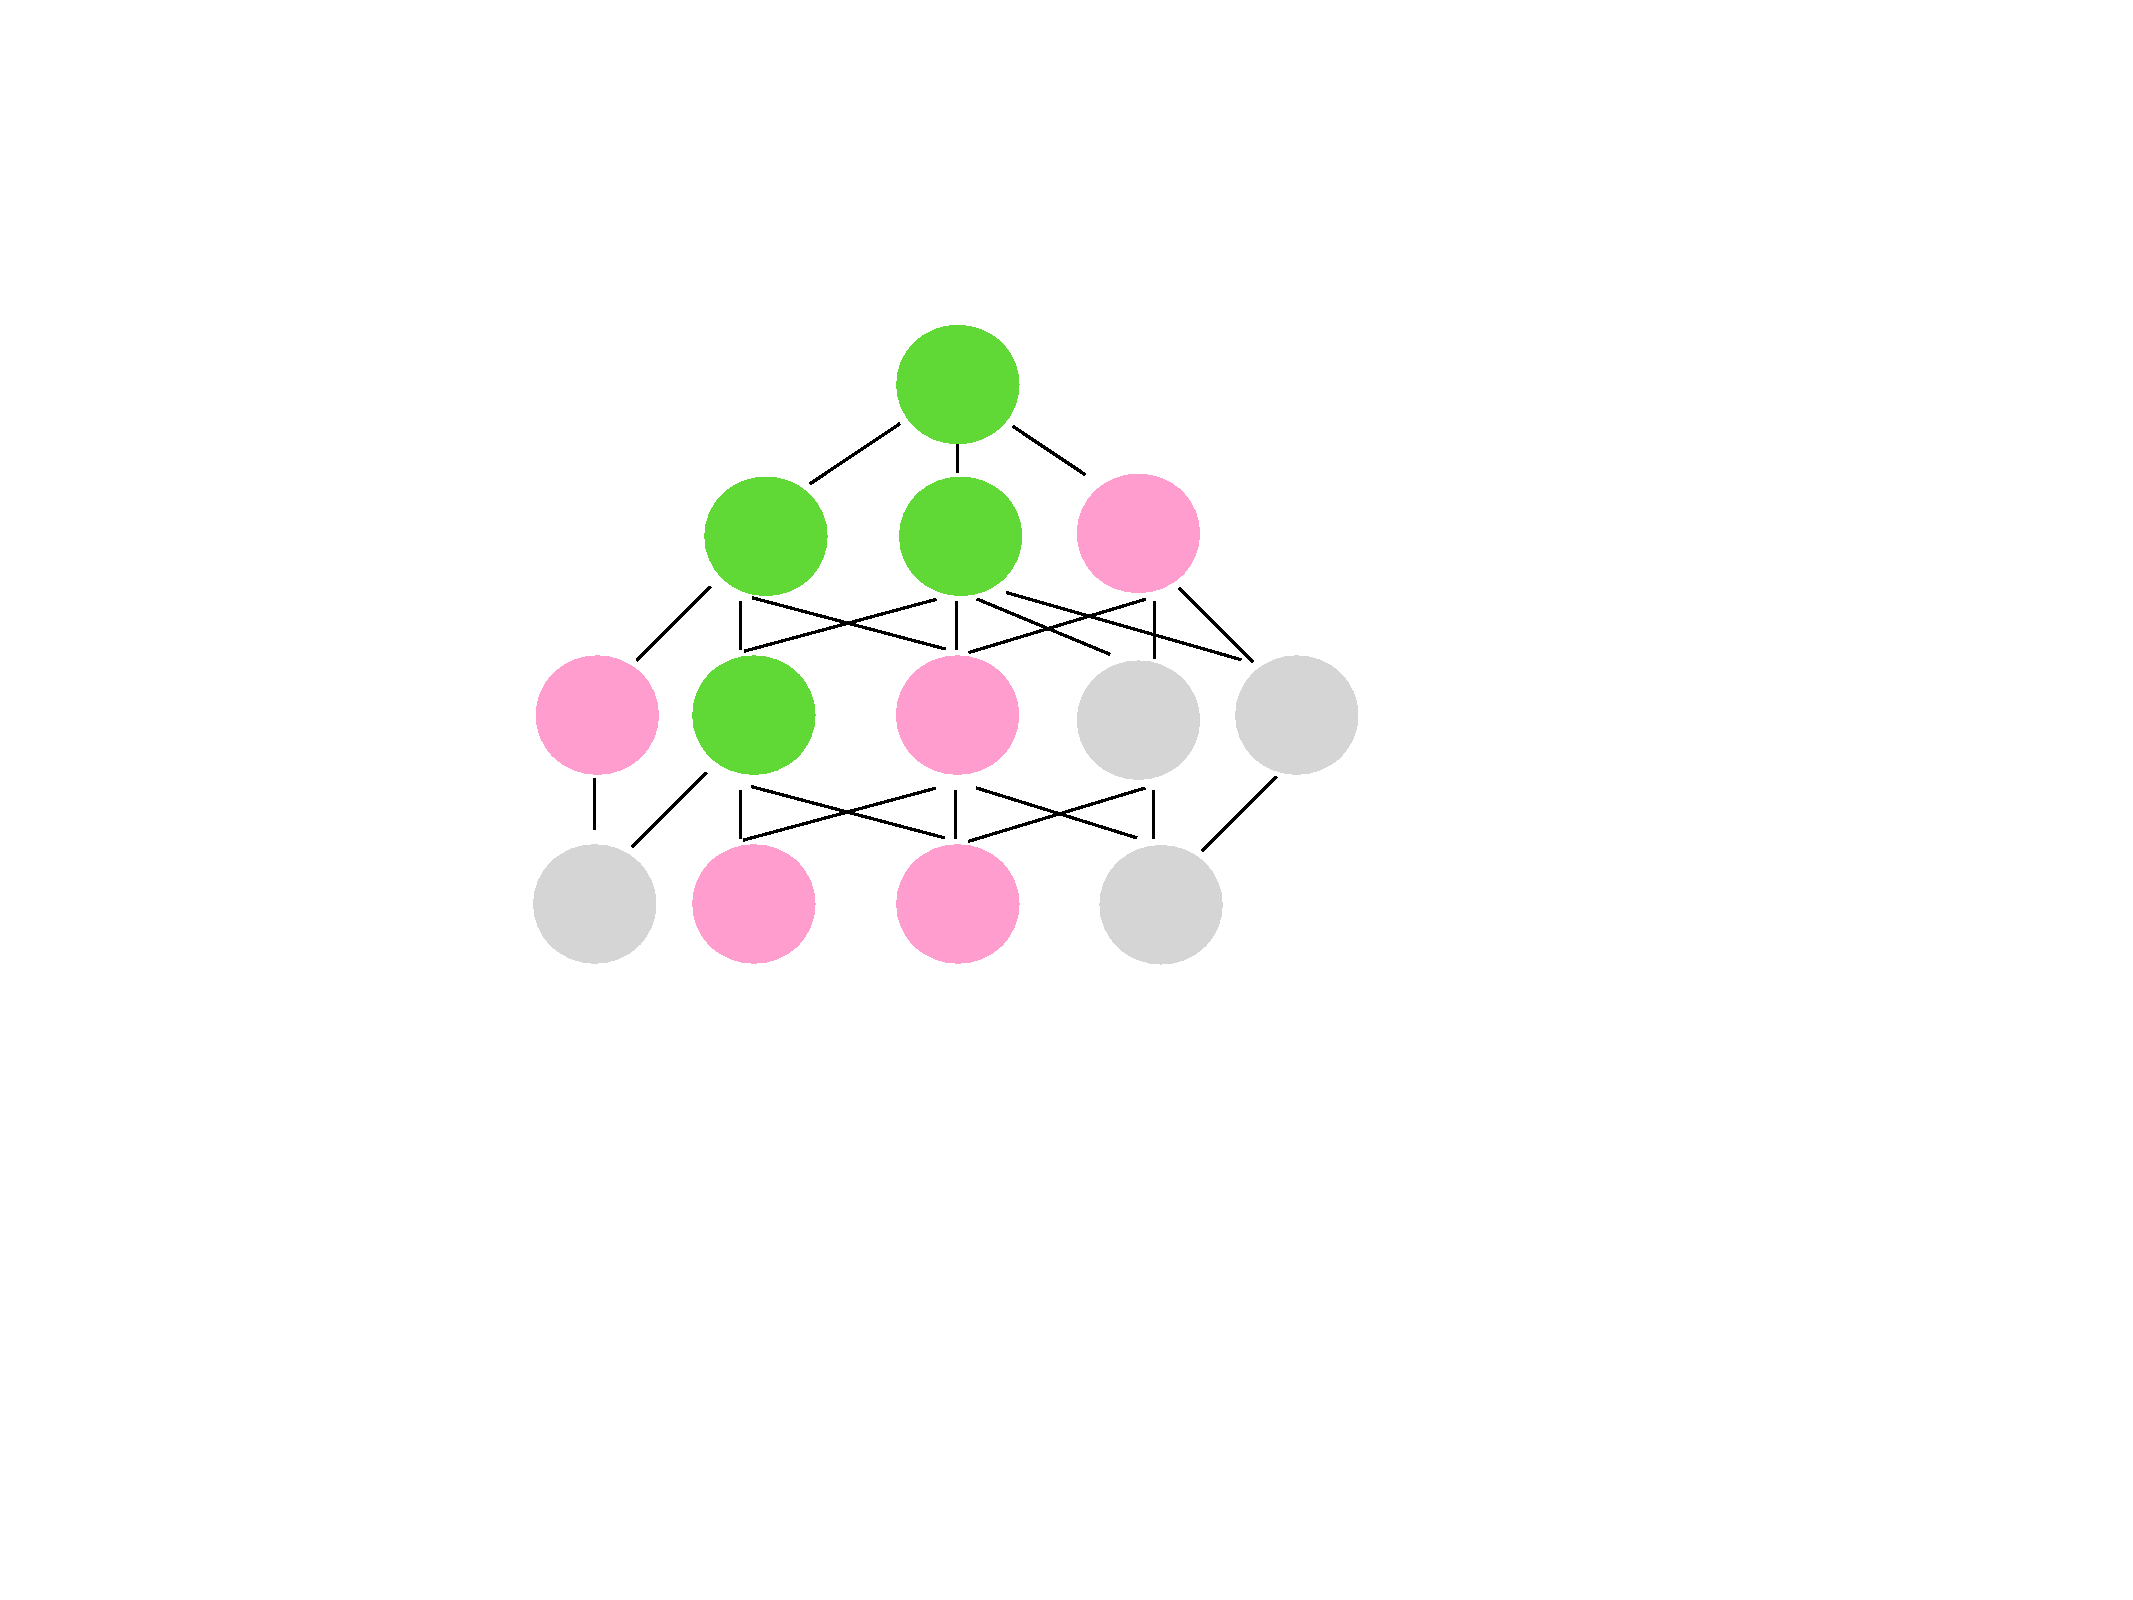
\includegraphics[width=0.4\linewidth]{figures/frontier.pdf}
% \caption{Toy example demonstrating the notion of ``frontier''. Nodes that have been picked to include in the dashboard are colored green. The neighbors of the set of picked nodes are the frontier nodes, shown in pink. Grey nodes are other unpicked nodes in the lattice.}
% \end{figure}
%We devised two classes of heuristics algorithms, namely, frontier-based algorithms, and path-merging algorithms. These algorithms are guaranteed to find a solution that satisfies the constraints of our problem, except for the optimality.
\techreport{The frontier-based algorithms traverse the lattice from root to downwards, incrementally adding new nodes (visualizations) to the current solution (dashboard) till it reaches the maximum capacity $k$. To achieve this, the algorithms maintain a list of candidate nodes---called \textit{frontier} nodes---any of which can be added to the current solution since their informative parent is already present in the solution. At each step, the algorithms add a node from frontier to the current solution, and update the frontier accordingly.  The frontier based algorithms can be further categorized into three types based on their node selection strategy (from frontier), namely greedy algorithm, random walk algorithm, and probabilistic algorithm. The greedy algorithm picks the current best node from frontier (thus concentrates on exploitation), random walk algorithm picks a random node (thus concentrates on exploration), and probabilistic algorithm picks a random high-utility node (thus trades off between exploration and exploitation).}
\par As described in Algorithm \ref{algo:frontier_greedy}, our algorithm obtains a list of candidate nodes known as the \textit{frontier} nodes (pink in Figure\ref{fig:lattice} left), which encompasses all neighbors of nodes in the existing subgraph solution. Any of the nodes in the frontier can be added to the current solution since their informative parent is guaranteed to be present in the solution. The \texttt{getFrontier} function scans and adds all children of leaf nodes of the current dashboard as part of the frontier. In the online version, it additionally checks for each child whether its informative parent is present in the current dashboard. At each step, our algorithm greedily picks the node with the maximum utility from the frontier to the current solution, and updates the frontier accordingly.

\techreport{The path merging algorithm first generate the informative paths from root to every candidate node. Then, it greedily merges the paths with high-utility to create a subgraph whose size is less than or equal to maximum capacity $k$.}

% \begin{algorithm}
%     \SetKwInOut{Input}{Input}
%     \SetKwInOut{Output}{Output}
%     \Input{Precomputed Lattice of Visualizations, $G = \{V_1, \ldots, V_n\}$}
%     \Output{A Dashboard of Size $k$, $S$}
%     $S = \{ V_{root}\}$\;
%     $F = get\_child(V_{root})$\;
%     \While{$size(S) < k$}
%     {
%     	$s_{next} = pick\_next(F)$\;
%     	$S = S \cup s_{next}$\;
%       \For{$i = 0;\ i < size(S);\ i = i + 1$}
%       {
%           $F = (F \cup get\_child(S[i])) - S$\;
%       }
%     }
%     return $S$\;
%     \caption{Frontier Based Algorithm}
% \end{algorithm}

\begin{algorithm}
  \begin{algorithmic}[1]
  \Procedure{pickVisualizations}{k,lattice}
  \State dashboard $\gets$ \{ $V_{overall}$ \}
  \While{|dashboard| < k}
      \State frontier $\gets$ getFrontier(dashboard,lattice)
      \State maxNode $\gets$ getMaxUtilityNode(frontier)
      \State dashboard $\gets$ dashboard $\cup$ \{maxNode\}
  \EndWhile
  \Return dashboard
  \EndProcedure
  \end{algorithmic}
  \caption{Frontier Greedy Algorithm}\label{algo:frontier_greedy}
\end{algorithm}

%\textbf{Greedy Algorithms:} Greedy algorithms select the locally optimal node to be added to the frontier.

%A specific implementation would need to specify a scoring function to nodes in frontier that is used to pop out the next node in each iteration. One can design a scoring function based on the trade-off between performance and complexity. In the most simple case, we can use the edge weights to score nodes in the frontier. That is, at each point we add a node with the highest interestingness value. We note that this is quite a greedy approach. Specifically, we might miss visualizations with high utility that are in deeper levels of the graph. Thus, another approach would be to extent the horizon for which we calculate a nodes utility. We denote such approach as a look-ahead approach. With a free parameter $n$, we would like to assign a score to each frontier node the corresponds to the expected utility of adding this node and $n-1$ more nodes who are its descendants. For example, we can run BFP for each node in frontier treating it as a root.

\techreport{The path merging algorithm first generate the informative paths from root to every candidate node. Then, it greedily merges the paths with high-utility to create a subgraph whose size is less than or equal to maximum capacity $k$.}
